

%-------------------------------------------------------------------------------
% Dokumenten Klasse
\documentclass[
	final,
	a4paper,
	oneside,
	parskip=full,
	headings=standardclasses,
	headings=big,
	pointednumbers,
    fleqn
]{scrartcl}

%-------------------------------------------------------------------------------
% Packete nutzen
\usepackage{ngerman,palatino,setspace}
\usepackage[T1]{fontenc}
\usepackage[utf8]{inputenc}
\usepackage[left=20mm,right=20mm,top=10mm,bottom=25mm]{geometry}
\usepackage{amsmath}
\usepackage{amssymb}
\usepackage{mathtools}

%-------------------------------------------------------------------------------
\usepackage[dvipsnames]{xcolor}

%-------------------------------------------------------------------------------
% dbox
\usepackage{dashbox}

%-------------------------------------------------------------------------------
% uline
\usepackage{ulem}

%-------------------------------------------------------------------------------
% TikZ
\usepackage{tikz}
%\usetikzlibrary{positioning, arrows, decorations}
\usetikzlibrary{
    trees,
    shapes,
    arrows,
    backgrounds,
    positioning,
    fit,
    petri,
    decorations,
    decorations.pathmorphing,
    decorations.pathreplacing
}

\tikzset{
    myptr/.style={
        ->,
        >=stealth
    }
}

\newcommand{\tikzmark}[1]{\tikz[overlay,remember picture,baseline=(#1.base)] \node (#1) {\strut};}


%-------------------------------------------------------------------------------
% \ifthenelse
\usepackage{ifthen}

%-------------------------------------------------------------------------------
% Für enumerate
\usepackage{enumitem}
\setlist[enumerate]{
    wide=0pt,
    leftmargin=*,
    itemsep=-1ex,
    parsep=2ex,
    labelsep=1ex,
    label=\alph*)
}

\usepackage{multirow}
\usepackage{ifthen}

%-------------------------------------------------------------------------------
% tabu
\usepackage{tabu} 

%-------------------------------------------------------------------------------
% tabu
%\usepackage{tabularx}
\usepackage{array}

%-------------------------------------------------------------------------------
% table line breaks with \makecell
\usepackage{makecell}
\renewcommand\cellalign{bl}

%-------------------------------------------------------------------------------
% 
\usepackage{xparse}
% 1: Subscription  (default: '')
% 2: Funktion Name (default: 'f')
% 3: Argument      (default: 'x')
% \fx         = f(x)
% \fx[1]      = f_1(x)
% \fx[][u]    = u(x)
% \fx[][u][x] = u(x)
% \fx[][f][u] = f(u)
\NewDocumentCommand{\fx}{ O{} O{f} O{x} }{{#2_{#1}{\left( #3 \right)}}}
\NewDocumentCommand{\dfx}{ O{} O{f} O{x} }{{#2'_{#1}{\left( #3 \right)}}}
\NewDocumentCommand{\dx}{ O{} }{{\Delta x^{#1}}}
\NewDocumentCommand{\dy}{ O{} }{{\Delta y^{#1}}}
\NewDocumentCommand{\dt}{ O{} }{{\Delta t^{#1}}}
\NewDocumentCommand{\du}{ O{} }{{\Delta u^{#1}}}
\NewDocumentCommand{\px}{ O{} }{{\partial x^{#1}}}
\NewDocumentCommand{\py}{ O{} }{{\partial y^{#1}}}
\NewDocumentCommand{\pt}{ O{} }{{\partial t^{#1}}}
\NewDocumentCommand{\pu}{ O{} }{{\partial u^{#1}}}
\NewDocumentCommand{\p}{ O{} }{{\partial^{#1}}}
\NewDocumentCommand{\re}{ O{} }{{\mathbb{R}^{#1}}}

\NewDocumentCommand{\xyz}{ O{x} O{y} O{z} }{#1 #2 #3}
% 1: Value
% 2: Key
% 3: Background Color
\NewDocumentCommand{\tfill}{ O{} O{} O{blue!20} }{%
    \tikz[baseline, every node/.style={inner sep=3pt,outer sep=0pt,minimum width=3mm,minimum height=4mm}]{
        \node[fill=#3,anchor=base] (#2) {#1};
    }
}
\NewDocumentCommand{\tfillc}{ O{} O{} }{%
    \tikz[baseline, every node/.style={inner sep=2pt,outer sep=0pt}]{
        \node[fill=#2,anchor=base] {#1};
    }
}

\NewDocumentCommand{\tdrawc}{ O{} O{} }{%
    \tikz[baseline, every node/.style={inner sep=2pt,outer sep=0pt}]{
        \node[rectangle,draw=#2,anchor=base] {#1};
    }
}

\NewDocumentCommand{\tcrossc}{ O{} O{} }{%
    \tikz[baseline, every node/.style={inner sep=0pt,outer sep=0pt}]{
        \node[draw=#2,anchor=base,strike out,line width=1pt] {#1};
    }
}

\newcommand{\tfillb}[1]{\tfillc[#1][blue!20]}
\newcommand{\tfillo}[1]{\tfillc[#1][orange!40]}
\newcommand{\tfillg}[1]{\tfillc[#1][Green!20]}
\newcommand{\tfilly}[1]{\tfillc[#1][yellow!40]}
\newcommand{\tfillr}[1]{\tfillc[#1][red!20]}
\newcommand{\tfillv}[1]{\tfillc[#1][Violet!20]}
\newcommand{\tfillt}[1]{\tfillc[#1][Turquoise!20]}
\newcommand{\tfillgr}[1]{\tfillc[#1][Gray!20]}


\newcommand{\tdrawb}[1]{\tdrawc[#1][blue!40]}
\newcommand{\tdrawo}[1]{\tdrawc[#1][orange!60]}
\newcommand{\tdrawg}[1]{\tdrawc[#1][Green!40]}
\newcommand{\tdrawy}[1]{\tdrawc[#1][yellow!60]}
\newcommand{\tdrawr}[1]{\tdrawc[#1][red!40]}
\newcommand{\tdrawv}[1]{\tdrawc[#1][Violet!40]}
\newcommand{\tdrawt}[1]{\tdrawc[#1][Turquoise!40]}
\newcommand{\tdrawgr}[1]{\tdrawc[#1][Gray!40]}
\newcommand{\tdrawk}[1]{\tdrawc[#1][black]}


\newcommand{\tcrossr}[1]{\tcrossc[#1][red]}
\newcommand{\tcrossg}[1]{\tcrossc[#1][green]}
\newcommand{\tcrossb}[1]{\tcrossc[#1][blue]}

% 1: Funktion Name
% 2: dx
% 3: dx^2
% 4: x_1
% 5: x_2
% 5: x_3
\NewDocumentCommand{\gpp}{ O{} O{\dx} O{\dx[2]} O{x} O{x} O{x} }{%
    \frac{1}{#3}
    \kl{#1 
        \kl{#4 \ifthenelse{\equal{#2}{}}{}{+ #2}} - 
        2 \cdot #1\kl{#5} +
        #1 \kl{#6\ifthenelse{\equal{#2}{}}{}{- #2}}
    }
}

% 1: x_1
% 2: x_2
% 3: x_3
% 4: dx^2
\NewDocumentCommand{\gppn}{ O{x_1} O{x_2} O{x_3} O{?}}{%
    \frac{1}{#4}
    \kl{#1 - 2 \cdot #2 + #3}
}

\newcommand*\difx{\; \mathop{}\!\mathrm{d}x}
\newcommand{\f}[2]{\frac{#1}{#2}}
%\newcommand{\fs}[2]{{\scriptstyle\frac{#1}{#2}}}
\newcommand{\fs}[2]{{\tfrac{#1}{#2}}}
\newcommand{\kl}[1]{{\left( #1 \right)}}
\newcommand{\kq}[1]{{\left\{ #1 \right\}}}
\newcommand{\ks}[1]{{\left[ #1 \right]}}


\newcommand{\dom}{{\Omega}}
\newcommand{\bound}{{\partial \Omega}}
\newcommand{\e}{\mathrm{e}}
\newcommand{\lap}{\mathcal{L}}
\newcommand{\ddt}{\mathrm{d}t}
\newcommand{\aligntab}[1]{{$\!\begin{aligned}[t] #1 \end{aligned}$}}



%-------------------------------------------------------------------------------
% Dokument
\begin{document}

    \subsection*{Ableitungsregeln}
    
    \renewcommand{\arraystretch}{1.25}
    \begin{tabular}{lll}
        Faktorregel  & $ y = C \cdot \fx$                   & $ y' = C \cdot \dfx $ \\
                     & $ y = 5 \cdot x^2 $                  & $ y' = 5 \cdot 2 \cdot x$ \\
        Summenregel  & $ y = \fx[1] + \ldots +  \fx[n] $    & $ y' = \dfx[1] + \ldots + \dfx[n] $\\
                     & $ y = x^2 + x^3$                     & $ y' = 2 \cdot x + 3 \cdot x^2$ \\
        Produktregel & $ y = \fx[][u] \cdot \fx[][v] $      & $ y' = \fx[][u] \cdot \dfx[][v] + \dfx[][u] \cdot \fx[][v] $ \\
                     & $ y = x^2 \cdot e^{2x}  $            & $ y' = x^2 \cdot 2\cdot e^{2x} + 2\cdot x \cdot e^{2x} $ \\
                     &                                      & $ y' = {\left( 2x^2 + 2x \right)} e^{2x} $ \\
        Kettenregel  & $ y = f\kl{u\kl{x}} $                & $ y' = \dfx[][f][u] \cdot \dfx[][u][x] $ \\
                     & $ y = f\kl{x^2 - 5}, \; f = x^2 $    & $ y' = 2 u \cdot 2x = 4x \kl{x^2 - 5} $ \\
                     & $ y = \ln\kl{1 + x^2} $              & $ y' = \frac{1}{u} \cdot 2x = \frac{2x}{1 + x^2} $ \\
    \end{tabular} \\

    \renewcommand{\arraystretch}{1.25}
    \begin{tabular}{lll}
        Bestimmtes Integral & $ \int\limits_{a}^{b}{f\kl{x} \difx} $                      & $ = \ks{F\kl{x}}_{a}^{b} = F\kl{b} - F\kl{a} $ \\
        Faktorregel         & $ \int\limits_{a}^{b}{C \cdot f\kl{x} \difx} $              & $ = C \cdot \int\limits_{a}^{b}{f\kl{x} \difx} $     \\
        Summenregel         & $ \int\limits_{a}^{b}{\ks{f_1\kl{x} + f_2\kl{x}} \difx} $   & $ = \int\limits_{a}^{b}{f_1\kl{x} \difx} + \int\limits_{a}^{b}{f_2\kl{x} \difx} $      \\
        Zerlegungsregel     & $ \int\limits_{a}^{c}{f\kl{x} \difx} $                      & $ = \int\limits_{a}^{b}{f\kl{x} \difx} + \int\limits_{b}^{c}{f\kl{x} \difx}$  \\
    \end{tabular} \\

    %===================================================================================
    \newpage

    \begin{flalign*}
        s \mapsto F\kl{s} = \lap \kq{f}\kl{s} = \int\limits_{0}^{\infty} f\kl{t} \cdot e^{-st} \cdot \ddt & &
    \end{flalign*}
    \begin{enumerate}
        \item{\begin{tabular}[t]{l}
                $f\kl{t} = a$ \\ \\
                {$\!\begin{aligned}[t]
                    % line 1
                    \int\limits_{0}^{\infty} a \cdot e^{-st} \cdot \ddt &=
                    \ks{ a \cdot \f{1}{-s} \cdot \e^{-st}}_{0}^{\infty} \\
                    % line 2
                    &= \ks{\kl{a \cdot \f{1}{-s} \cdot \tikzmark{p1l}\e^{-s\infty}\tikzmark{p1r}} - \kl{a \cdot \f{1}{-s} \cdot \tikzmark{p2l}\e^{-s0}\tikzmark{p2r}} } \\[1.5em]
                    % line 3
                    &= \ks{\kl{0} - \kl{a \cdot \f{1}{-s}}} \\[1em]
                    % line 4
                    &= \f{a}{s}
                \end{aligned}
                \def\yshift{2pt}
                \tikz[overlay, remember picture, decoration={brace, amplitude=3pt}] {
                   \draw[decorate] ([yshift=\yshift]p1r.south) -- ([yshift=\yshift]p1l.south)
                       node [midway,below=5pt] {$0$};
                   \draw[decorate] ([yshift=\yshift]p2r.south) -- ([yshift=\yshift]p2l.south)
                       node [midway,below=5pt] {$1$};
                }$}
            \end{tabular}
        }
        \item{\begin{tabular}[t]{l}
                $f\kl{t} = \e^{-ct}$ \\ \\
                {$\!\begin{aligned}[t]
                    % line 1
                    \int\limits_{0}^{\infty} \e^{-ct} \cdot e^{-st} \cdot \ddt &=
                    \int\limits_{0}^{\infty} \e^{-ct-st} \cdot \ddt \\
                    % line 2
                    &= \int\limits_{0}^{\infty} \e^{\kl{-c-s}t} \cdot \ddt \\
                    % line 3
                    &= \ks{\f{1}{-c-s} \cdot \e^{\kl{-c-s}t}}_{0}^{\infty} \\
                    % line 4
                    &= \ks{\kl{\f{1}{-c-s} \cdot \tikzmark{p1l}\e^{\kl{-c-s}\infty}\tikzmark{p1r}} - \kl{\f{1}{-c-s} \cdot \tikzmark{p2l}\e^{\kl{-c-s}0}\tikzmark{p2r}}} \\[1.5em]
                    % line 5
                    &= \ks{\kl{0} - \kl{\f{1}{-c-s}}} \\
                    % line 6
                    &= \f{1}{c+s}
                \end{aligned}
                \def\yshift{2pt}
                \tikz[overlay, remember picture, decoration={brace, amplitude=3pt}] {
                   \draw[decorate] ([yshift=\yshift]p1r.south) -- ([yshift=\yshift]p1l.south)
                       node [midway,below=5pt] {$0$};
                   \draw[decorate] ([yshift=\yshift]p2r.south) -- ([yshift=\yshift]p2l.south)
                       node [midway,below=5pt] {$1$};
                }$}
            \end{tabular}
        }
        \item{\begin{tabular}[t]{l}
                $f\kl{t} = t$ \\ \\
                {$\!\begin{aligned}[t]
                    % line 1
                    \int\limits_{0}^{\infty} \tikzmark{p1l} \; \; t \; \; \tikzmark{p1r} \cdot \tikzmark{p2l} e^{-st} \tikzmark{p2r} \cdot \ddt &=
                    \ks{\; \; \tikzmark{p3l} \; \; t \; \; \tikzmark{p3r} \cdot \tikzmark{p4l} \f{1}{-s} \cdot \e^{-st} \tikzmark{p4r} \; \; }_{0}^{\infty} -
                    \int\limits_{0}^{\infty} \tikzmark{p5l} \; \; 1 \; \; \tikzmark{p5r} \cdot \tikzmark{p6l} \f{1}{-s} \cdot \e^{-st} \tikzmark{p6r} \cdot \ddt \\[1em]
                    % line 2
                    &= \ks{\kl{\infty \cdot \f{1}{-s} \cdot \tikzmark{p7l} \e^{-s\infty} \tikzmark{p7r} \; \;} - 
                    \kl{0 \cdot \f{1}{-s} \cdot \tikzmark{p8l} \e^{-s0} \tikzmark{p8r} \; \;} } -
                    \ks{\f{1}{-s} \cdot \f{1}{-s} \cdot \e^{-st} }_{0}^{\infty} \\[1.9em]
                    % line 3
                    &= \ks{0} - \ks{\kl{\f{1}{s^2} \cdot \e^{-s\infty} } - \kl{\f{1}{s^2} \cdot \e^{-s0} }} \\
                    &= \f{1}{s^2}
                \end{aligned}
                \def\yshift{-2pt}
                \tikz[overlay, remember picture, decoration={brace, amplitude=3pt}] {
                   \draw[decorate] ([yshift=\yshift]p1r.south) -- ([yshift=\yshift]p1l.south)
                       node [midway,below=5pt] {$u$};
                   \draw[decorate] ([yshift=\yshift]p2r.south) -- ([yshift=\yshift]p2l.south)
                       node [midway,below=2pt] {$v'$};
                   \draw[decorate] ([yshift=\yshift]p3r.south) -- ([yshift=\yshift]p3l.south)
                       node [midway,below=5pt] {$u$};
                   \draw[decorate] ([yshift=\yshift]p4r.south) -- ([yshift=\yshift]p4l.south)
                       node [midway,below=5pt] {$v$};
                   \draw[decorate] ([yshift=\yshift]p5r.south) -- ([yshift=\yshift]p5l.south)
                       node [midway,below=2pt] {$u'$};
                   \draw[decorate] ([yshift=\yshift]p6r.south) -- ([yshift=\yshift]p6l.south)
                       node [midway,below=5pt] {$v$};
                   \draw[decorate] ([yshift=\yshift]p7r.south) -- ([yshift=\yshift]p7l.south)
                       node [midway,below=5pt] {$0$};
                   \draw[decorate] ([yshift=\yshift]p8r.south) -- ([yshift=\yshift]p8l.south)
                       node [midway,below=5pt] {$1$};
                }$}
            \end{tabular}
        }
        \item{\begin{tabular}[t]{l}
                $f\kl{t} = g'\kl{t}$ \\ \\
                {$\!\begin{aligned}[t]
                    % line 1
                    \int\limits_{0}^{\infty} \tikzmark{p1l}g'\kl{t}\tikzmark{p1r} \cdot \tikzmark{p2l} \e^{-st} \tikzmark{p2r} \cdot \ddt
                    &= \ks{ \;
                        \tikzmark{p3l}g\kl{t}\tikzmark{p3r} \cdot \tikzmark{p4l} \e^{-st} \tikzmark{p4r}
                    \; }_{0}^{\infty} -
                    \int\limits_{0}^{\infty} \tikzmark{p5l}g\kl{t}\tikzmark{p5r} \cdot \tikzmark{p6l} \kl{-s} \cdot \e^{-st} \tikzmark{p6r} \cdot \ddt \\
                    % line 2
                    &= \ks{\kl{ g\kl{\infty} \cdot \tikzmark{p7l}\e^{-s\infty}\tikzmark{p7r}} - \kl{ g\kl{0} \cdot \tikzmark{p8l}\e^{-s0}\tikzmark{p8r}}} + s \cdot \int\limits_{0}^{\infty} g\kl{t} \cdot \e^{-st} \cdot \ddt \\[1em]
                    % line 3
                    &= - g\kl{0} + s \cdot \lap \kq{g}\kl{s}
                \end{aligned}
                \def\yshift{2pt}
                \tikz[overlay, remember picture, decoration={brace, amplitude=3pt}] {
                   \draw[decorate] ([yshift=\yshift]p1r.south) -- ([yshift=\yshift]p1l.south)
                       node [midway,below=2pt] {$u'$};
                   \draw[decorate] ([yshift=\yshift]p2r.south) -- ([yshift=\yshift]p2l.south)
                       node [midway,below=5pt] {$v$};
                   \draw[decorate] ([yshift=\yshift]p3r.south) -- ([yshift=\yshift]p3l.south)
                       node [midway,below=5pt] {$u$};
                   \draw[decorate] ([yshift=\yshift]p4r.south) -- ([yshift=\yshift]p4l.south)
                       node [midway,below=5pt] {$v$};
                   \draw[decorate] ([yshift=\yshift]p5r.south) -- ([yshift=\yshift]p5l.south)
                       node [midway,below=5pt] {$u$};
                   \draw[decorate] ([yshift=\yshift]p6r.south) -- ([yshift=\yshift]p6l.south)
                       node [midway,below=2pt] {$v'$};
                   \draw[decorate] ([yshift=\yshift]p7r.south) -- ([yshift=\yshift]p7l.south)
                       node [midway,below=5pt] {$0$};
                   \draw[decorate] ([yshift=\yshift]p8r.south) -- ([yshift=\yshift]p8l.south)
                       node [midway,below=5pt] {$1$};
                }$}
            \end{tabular}
        }
        \item{\begin{tabular}[t]{l}
                $f\kl{t} = g^{\kl{4}}\kl{t}$ \\ \\
                {$\!\begin{aligned}[t]
                    % line 1
                    \int\limits_{0}^{\infty} \tikzmark{p1l}g^{\kl{4}}\kl{t}\tikzmark{p1r} \cdot \tikzmark{p2l} \e^{-st} \tikzmark{p2r} \cdot \ddt
                    &= \ks{ \;
                        \tikzmark{p3l}g^{\kl{3}}\kl{t}\tikzmark{p3r} \cdot \tikzmark{p4l} \e^{-st} \tikzmark{p4r}
                    \; }_{0}^{\infty} -
                    \int\limits_{0}^{\infty} \tikzmark{p5l}g^{\kl{3}}\kl{t}\tikzmark{p5r} \cdot \tikzmark{p6l} \kl{-s} \cdot \e^{-st} \tikzmark{p6r} \cdot \ddt \\
                    % line 2
                    &= \ks{0 - g^{\kl{3}}\kl{0}} + s \cdot \int\limits_{0}^{\infty} g^{\kl{3}}\kl{t} \cdot \e^{-st} \cdot \ddt \\
                    % line 3
                    &= - g^{\kl{3}}\kl{0} + s \cdot \ks{
                        \ks{ \; g^{\kl{2}}\kl{t} \cdot \e^{-st} \; }_{0}^{\infty} -
                        \int\limits_{0}^{\infty} g^{\kl{2}}\kl{t} \cdot \kl{-s} \cdot \e^{-st} \cdot \ddt
                    } \\
                    % line 4
                    &= - g^{\kl{3}}\kl{0} -
                        s \cdot g^{\kl{2}}\kl{0} +
                        s^2 \cdot \int\limits_{0}^{\infty} g^{\kl{2}}\kl{t} \cdot \e^{-st} \cdot \ddt
                    \\
                    % line 5
                    &= - g^{\kl{3}}\kl{0} -
                        s \cdot g^{\kl{2}}\kl{0} -
                        s^2 \cdot g^{\kl{1}}\kl{0} +
                        s^3 \cdot \int\limits_{0}^{\infty} g^{\kl{1}}\kl{t} \cdot \e^{-st} \cdot \ddt
                    \\
                    % line 6
                    &= - g^{\kl{3}}\kl{0} -
                        s \cdot g^{\kl{2}}\kl{0} -
                        s^2 \cdot g^{\kl{1}}\kl{0} -
                        s^3 \cdot g\kl{0} +
                        s^4 \cdot \int\limits_{0}^{\infty} g\kl{t} \cdot \e^{-st} \cdot \ddt
                    \\
                    % line 6
                    &= - g^{\kl{3}}\kl{0} -
                        s \cdot g^{\kl{2}}\kl{0} -
                        s^2 \cdot g^{\kl{1}}\kl{0} -
                        s^3 \cdot g\kl{0} +
                        s^4 \cdot G\kl{s}
                    \\
                \end{aligned}
                \def\yshift{2pt}
                \tikz[overlay, remember picture, decoration={brace, amplitude=3pt}] {
                   \draw[decorate] ([yshift=\yshift]p1r.south) -- ([yshift=\yshift]p1l.south)
                       node [midway,below=2pt] {$u'$};
                   \draw[decorate] ([yshift=\yshift]p2r.south) -- ([yshift=\yshift]p2l.south)
                       node [midway,below=5pt] {$v$};
                   \draw[decorate] ([yshift=\yshift]p3r.south) -- ([yshift=\yshift]p3l.south)
                       node [midway,below=5pt] {$u$};
                   \draw[decorate] ([yshift=\yshift]p4r.south) -- ([yshift=\yshift]p4l.south)
                       node [midway,below=5pt] {$v$};
                   \draw[decorate] ([yshift=\yshift]p5r.south) -- ([yshift=\yshift]p5l.south)
                       node [midway,below=5pt] {$u$};
                   \draw[decorate] ([yshift=\yshift]p6r.south) -- ([yshift=\yshift]p6l.south)
                       node [midway,below=2pt] {$v'$};
                }$}
            \end{tabular}
        }
    \end{enumerate}

    %===================================================================================
    \newpage

    {\renewcommand{\arraystretch}{1.5}
    \begin{tabular}[t]{p{1.9cm}l}
        DGL:    & \aligntab{\f{\pu}{\tfillgr{$\pt$}} = \kappa \cdot \f{\p[2]u}{\px[2]}} \\
        Domain: & \aligntab{\dom = \kl{0,l} \times \re^{+}} \\
        Boundary Condition:     & \aligntab{
            u\kl{x,\tfillgr{$0$}} &= f\kl{x} \\
            u\kl{\tfillg{$0$},\tfillgr{$t$}} &= g_0\kl{\tfillgr{$t$}} \\
            \f{\p}{\px}u\kl{\tfilly{$l$},\tfillgr{$t$}} &= g_1\kl{\tfillgr{$t$}} \\
        } \\
        Laplace: & \aligntab{
            -u\kl{x,\tfillgr{$0$}} + s \cdot \lap u\kl{x,\tfillo{$s$}} &= \f{\p[2]}{\px[2]} \lap u\kl{x,\tfillo{$s$}} \\
            \f{\p[2]}{\px[2]} \lap u\kl{x,\tfillo{$s$}} - s \cdot \lap u\kl{x,\tfillo{$s$}} &= -u\kl{x,\tfillgr{$0$}} \\
            u\kl{x,\tfillgr{$0$}} &= f\kl{x} \\
            \lap u\kl{\tfillg{$0$},\tfillo{$s$}} &= \lap g_0\kl{\tfillo{$s$}} = G_0\kl{\tfillo{$s$}} \\
            \f{\p}{\px}\lap u\kl{\tfilly{$l$},\tfillo{$s$}} &= \lap g_1\kl{\tfillo{$s$}} = G_1\kl{\tfillo{$s$}} \\
            y_s''\kl{x} - s \cdot y_s\kl{x} &= -f\kl{x} \\
            y_s\kl{\tfillg{$0$}} &= G_0\kl{\tfillo{$s$}} \\
            y_s\kl{\tfilly{$l$}} &= G_1\kl{\tfillo{$s$}}
        } \\
        Values: & \begin{tabular}[t]{ll}
            \aligntab{u\kl{x,\tfillgr{$0$}} &= f\kl{x} = 0}                             & \aligntab{\Rightarrow y_s''\kl{x} - s \cdot y_s\kl{x} = 0} \\
            \aligntab{u\kl{\tfillg{$0$},\tfillgr{$t$}} &= g_0\kl{\tfillgr{$t$}} = 0}           & \aligntab{\Rightarrow y_s\kl{\tfillg{$0$}} = 0} \\
            \aligntab{\f{\p}{\px}u\kl{\tfilly{$l$},\tfillgr{$t$}} &= g_1\kl{\tfillgr{$t$}} = 1} & \aligntab{\Rightarrow y_s'\kl{\tfilly{$l$}} = \f{1}{s}}
        \end{tabular} \\
        General Solution:& \begin{tabular}[t]{l}
            \texttt{deSolve($y''-s \cdot  y = 0$, x, y) $\mid$ s > 0} \\
            \aligntab{
                y_s\kl{x} &= A_s \cdot \e^{\sqrt{s} \cdot x} + B_s \cdot \e^{-\sqrt{s} \cdot x}\\
                &= \f{\tfillb{$k_1$} + \tfillr{$k_2$}}{2} \cdot \e^{\sqrt{s} \cdot x} + \f{\tfillb{$k_1$} - \tfillr{$k_2$}}{2} \cdot \e^{-\sqrt{s} \cdot x}\\
                &= \f{\tfillb{$k_1$} \cdot \e^{\sqrt{s} \cdot x} + \tfillr{$k_2$} \cdot \e^{\sqrt{s} \cdot x} + \tfillb{$k_1$} \cdot \e^{-\sqrt{s} \cdot x} - \tfillr{$k_2$} \cdot \e^{-\sqrt{s} \cdot x}}{2}\\
                &= \tfillb{$k_1$} \cdot \f{1}{2} \kl{\e^{\sqrt{s} \cdot x} + \e^{-\sqrt{s} \cdot x}} + \tfillr{$k_2$} \cdot \f{1}{2} \kl{\e^{\sqrt{s} \cdot x} - \e^{-\sqrt{s} \cdot x}}\\
                &= \tfillb{$k_1$} \cdot \cosh\kl{\sqrt{s} \cdot x} + \tfillr{$k_2$} \cdot \sinh\kl{\sqrt{s} \cdot x}
            }
        \end{tabular} \\
        Particular Solution:& \aligntab{
                y_s\kl{x} &= k_1 \cdot \cosh\kl{\sqrt{s} \cdot x} + k_2 \cdot \sinh\kl{\sqrt{s} \cdot x} \\
                y_s\kl{\tfillg{$0$}} &= k_1 \cdot \tikzmark{p1l}\cosh\kl{\sqrt{s} \cdot \tfillg{$0$}}\tikzmark{p1r} + k_2 \cdot \tikzmark{p2l}\sinh\kl{\sqrt{s} \cdot \tfillg{$0$}} \tikzmark{p2r} = 0\\[1em]
                &\Rightarrow k_1 = 0 \\
                y_s\kl{x} &= k_2 \cdot \sinh\kl{\sqrt{s} \cdot x} \\
                y_s'\kl{x} &= k_2 \cdot \sqrt{s} \cdot \sinh\kl{\sqrt{s} \cdot x} \\
                y_s\kl{\tfilly{$l$}} &= k_2 \cdot \sqrt{s} \cdot \sinh\kl{\sqrt{s} \cdot \tfilly{$l$}} = \f{1}{s}\\
                &\Rightarrow k_2 = \f{1}{s \cdot \sqrt{s} \cdot \sinh\kl{\sqrt{s} \cdot \tfilly{$l$}}} \\
                y_s\kl{x} &= \f{1}{s \cdot \sqrt{s} \cdot \sinh\kl{\sqrt{s} \cdot \tfilly{$l$}}} \cdot \sinh\kl{\sqrt{s} \cdot x} = \lap u\kl{x,s}
        }{$\!
            \def\yshift{4pt}
            \tikz[overlay, remember picture, decoration={brace, amplitude=3pt}] {
               \draw[decorate] ([yshift=\yshift]p1r.south) -- ([yshift=\yshift]p1l.south)
                   node [midway,below=5pt] {$1$};
               \draw[decorate] ([yshift=\yshift]p2r.south) -- ([yshift=\yshift]p2l.south)
                   node [midway,below=5pt] {$0$};
            }
        $}
    \end{tabular}

    %===================================================================================
    \newpage

    {\renewcommand{\arraystretch}{1.5}
    \begin{tabular}[t]{p{1.9cm}l}
        DGL:                & \aligntab{ \f{\pu}{\px} + \f{\pu}{\tfillgr{$\pt$}} = 1} \\
        Domain:             & \aligntab{\dom = \kq{\kl{x,t} \mid t > 0}} \\
        Boundary Condition: & \aligntab{u\kl{x,\tfillgr{$0$}} &= g\kl{x}} \\
        Laplace: & \aligntab{
            \tikzmark{p1l} \f{\p}{\px} \lap u\kl{x,s}\tikzmark{p1r} + s \cdot \tikzmark{p2l}\lap u\kl{x,s} \tikzmark{p2r} -u \kl{x,\tfillgr{$0$}} &= \lap\kq{1} \\[1.5em]
        }{$\!
            \def\yshift{0pt}
            \tikz[overlay, remember picture, decoration={brace, amplitude=3pt}] {
               \draw[decorate] ([yshift=\yshift]p1r.south) -- ([yshift=\yshift]p1l.south)
                   node [midway,below=2pt] {$y_s'$};
               \draw[decorate] ([yshift=\yshift]p2r.south) -- ([yshift=\yshift]p2l.south)
                   node [midway,below=5pt] {$y_s$};
            }
        $} \\
        & \aligntab{
            y_s'\kl{x} + s \cdot y_s\kl{x} - g\kl{x} &= \f{1}{s}
        } \\
        General Solution:   & \begin{tabular}[t]{l}
            \texttt{deSolve($y'' + s \cdot  y = \f{1}{s} + g\kl{x}$, x, y) $\mid$ s > 0}\\
            \aligntab{
                y_s\kl{x} &= A_s \cdot \e^{- s \cdot x} + \f{g\kl{x} \cdot s}{s^2} + \f{1}{s^2}
            }
        \end{tabular} \\
        Charakter.: & \begin{tabular}[t]{lll}
            \multicolumn{3}{l}{\aligntab{\tfillr{$u_0$} = u\kl{\tfillg{$x_0$},\tfillb{$0$}} = g\kl{x_0}\\[0.5em]}}\\
            \aligntab{c = 
            \begin{pmatrix}
                1 \\
                1 \\
                1 
            \end{pmatrix}} &{\arraycolsep=2pt
            \aligntab{\begin{array}{rl}
                \dot{x} &= 1 \\
                \dot{t} &= 1 \\
                \dot{u} &= 1
            \end{array}}} &{\arraycolsep=2pt
            \aligntab{\begin{array}{rll}
                x &= \tau + \tfillg{$x_0$} &= \tau + x_0 \\
                t &= \tau + \tfillb{$t_0$} &= \tau\\
                u &= \tau + \tfillr{$u_0$} &= \tau + g\kl{x_0}
            \end{array}}} \\
            \multicolumn{3}{l}{{\arraycolsep=2pt
            \aligntab{\begin{array}{rl}
                \tau &= t\\
                x_0  &= x - t\\
                u    &= t + g\kl{x - t}
            \end{array}}}}
        \end{tabular}\\
            Insert \; \; Solution: &
            \aligntab{
                u\kl{x,t} &= t + g\kl{x - t} \\
                \p_x u\kl{x,t} &= g'\kl{x - t} \\
                y_s\kl{x} &=
                    \int\limits_{0}^{\infty} \kl{t + g\kl{x - t}} \cdot \e^{-st} \cdot \ddt \\
                    &= \int\limits_{0}^{\infty} t \cdot \e^{-st} \cdot \ddt +
                    \int\limits_{0}^{\infty} g\kl{x - t} \cdot \e^{-st} \cdot \ddt \\
                y_s'\kl{x} &=
                    \int\limits_{0}^{\infty} \tikzmark{p1l}g'\kl{x - t}\tikzmark{p1r} \cdot \tikzmark{p2l} \e^{-st} \tikzmark{p2r} \cdot \ddt \\
                    &= \ks{ \;
                        \tikzmark{p3l} - g\kl{x - t}\tikzmark{p3r} \cdot \tikzmark{p4l} \e^{-st} \tikzmark{p4r}
                    \; }_{0}^{\infty} -
                    \int\limits_{0}^{\infty} \tikzmark{p5l} - g\kl{x - t}\tikzmark{p5r} \cdot \tikzmark{p6l} \kl{-s} \cdot \e^{-st} \tikzmark{p6r} \cdot \ddt \\
                    &= \ks{ \; 0 - \kl{- g\kl{x - 0}} \; } -
                    s \cdot \int\limits_{0}^{\infty} g\kl{x - t} \cdot \e^{-st} \cdot \ddt \\
            }{$\!
            \def\yshift{0pt}
            \tikz[overlay, remember picture, decoration={brace, amplitude=3pt}] {
               \draw[decorate] ([yshift=\yshift]p1r.south) -- ([yshift=\yshift]p1l.south)
                   node [midway,below=2pt] {$u'$};
               \draw[decorate] ([yshift=\yshift]p2r.south) -- ([yshift=\yshift]p2l.south)
                   node [midway,below=5pt] {$v$};
               \draw[decorate] ([yshift=\yshift]p3r.south) -- ([yshift=\yshift]p3l.south)
                   node [midway,below=5pt] {$u$};
               \draw[decorate] ([yshift=\yshift]p4r.south) -- ([yshift=\yshift]p4l.south)
                   node [midway,below=5pt] {$v$};
               \draw[decorate] ([yshift=\yshift]p5r.south) -- ([yshift=\yshift]p5l.south)
                   node [midway,below=5pt] {$u$};
               \draw[decorate] ([yshift=\yshift]p6r.south) -- ([yshift=\yshift]p6l.south)
                   node [midway,below=2pt] {$v'$};
            }
        $} \\
        \multicolumn{2}{l}{\aligntab{
                & \tfillr{$y_s'\kl{x}$} + s \cdot \tfillg{$y_s\kl{x}$} - \tfillb{$g\kl{x}$} = &\\
                & \tdrawr{$\tcrossr{$g\kl{x}$} - \tcrossb{$s \cdot \int\limits_{0}^{\infty} g\kl{x - t} \cdot \e^{-st} \cdot \ddt$}$} +
                s \cdot \tdrawg{$\int\limits_{0}^{\infty} t \cdot \e^{-st} \cdot \ddt + \tcrossb{$\int\limits_{0}^{\infty} g\kl{x - t} \cdot \e^{-st} \cdot \ddt$}$} -
                \tdrawb{$\tcrossr{$g\kl{x}$}$} = & \\
                & \tfillgr{$s$} \cdot \int\limits_{0}^{\infty} t \cdot \e^{-st} \cdot \ddt =
                    \tfillgr{$s$} \cdot \ks{ t \cdot\f{1}{-s} \cdot \e^{-st} }_{0}^{\infty} -
                    \tfillgr{$s$} \cdot \int\limits_{0}^{\infty} 1 \cdot \f{1}{-s} \cdot \e^{-st} \cdot \ddt = & \\
                & \tfillgr{$s$} \cdot \ks{0} - \tfillgr{$s$} \cdot \ks{\f{1}{s^2} \cdot \e^{-st}}_{0}^{\infty} =
                    \tfillgr{$s$} \cdot \ks{0} - \tfillgr{$s$} \ks{\kl{0} - \kl{\f{1}{s^2} \cdot 1}} = \f{1}{s }&
            }
        }
    \end{tabular}

    %===================================================================================
    \newpage

    {\renewcommand{\arraystretch}{1.5}
    \begin{tabular}[t]{p{1.9cm}l}
        DGL:                & \aligntab{ \f{\p[4]u}{\p \tfillgr{$t^4$}} + \f{\pu}{\px} = 0} \\
        Domain:             & \aligntab{\dom = \kq{\kl{x,t} \mid t > 0 \; \text{and} \; x > 0}} \\
        Boundary Condition: & \aligntab{
                                u\kl{x,\tfillgr{$0$}} &= 0 \\
                                \f{\pu}{\pt} u\kl{x,\tfillgr{$0$}} &= 0 \\
                                \f{\p[2]u}{\pt[2]} u\kl{x,\tfillgr{$0$}} &= 0 \\
                                \f{\p[3]u}{\pt[3]} u\kl{x,\tfillgr{$0$}} &= 1 \\
                                u\kl{0,\tfillgr{$t$}} &= \e^{-t} \\[1em]
                              } \\
        Laplace: & \aligntab{
            & s^4 \cdot \tikzmark{p1l}\lap u\kl{x,s} \tikzmark{p1r} -
            s^3 \cdot \f{\p[3]u}{\pt[3]} u\kl{x,\tfillgr{$0$}} -
            s^2 \cdot \f{\p[2]u}{\pt[2]} u\kl{x,\tfillgr{$0$}} -  & \\
            & s \cdot \f{\pu}{\pt} u\kl{x,\tfillgr{$0$}} - 
            u \kl{x,\tfillgr{$0$}} +
            \tikzmark{p2l} \f{\p}{\px} \lap u\kl{x,s}\tikzmark{p2r} = \lap\kq{0} & \\[1.5em]
        }{$\!
            \def\yshifta{-4pt}
            \def\yshiftb{-2pt}
            \tikz[overlay, remember picture, decoration={brace, amplitude=3pt}] {
               \draw[decorate] ([yshift=\yshifta]p1l.north) -- ([yshift=\yshifta]p1r.north)
                   node [midway,above=2pt] {$y_s$};
               \draw[decorate] ([yshift=\yshiftb]p2r.south) -- ([yshift=\yshiftb]p2l.south)
                   node [midway,below=2pt] {$y_s'$};
            }
        $} \\
        & \aligntab{
            s^4 \cdot y_s\kl{x} - 1 + y_s'\kl{x} &= 0 \\
            y_s'\kl{x} + s^4 \cdot y_s\kl{x} &= 1 \\[1em]
        } \\
        & \aligntab{
            u\kl{0,\tfillgr{$t$}} &= \e^{-t} \Leftrightarrow \lap \kq{u\kl{0,s}} = y_s\kl{0} = \f{1}{s+1}
        }\\
        General Solution:   & \begin{tabular}[t]{l}
            \texttt{deSolve($y' + s^4 \cdot  y = 1$, x, y)}\\
            \aligntab{
                y_s\kl{x} &= A_s \cdot \e^{-s^4 \cdot x} + \f{1}{s^4}
            }
        \end{tabular} \\
        Particular Solution:& \aligntab{
                y_s\kl{0} &=A_s \cdot \tikzmark{p1l}\e^{-s^4 \cdot 0}\tikzmark{p1r} + \f{1}{s^4} = \f{1}{s+1} \\[1.5em]
                 & \Rightarrow A_s = \f{1}{s+1} - \f{1}{s^4} \\
                y_s\kl{x} &= \kl{\f{1}{s+1} - \f{1}{s^4}}\cdot \e^{-s^4 \cdot x} + \f{1}{s^4}
        }{$\!
            \def\yshift{4pt}
            \tikz[overlay, remember picture, decoration={brace, amplitude=3pt}] {
               \draw[decorate] ([yshift=\yshift]p1r.south) -- ([yshift=\yshift]p1l.south)
                   node [midway,below=5pt] {$1$};
            }
        $}
    \end{tabular}

    %===================================================================================
    \newpage

    {\renewcommand{\arraystretch}{1.75}
    \begin{tabular}{ll}
        Forward FDM  & $g'\kl{x} = \frac{g \kl{x + \dx} - g \kl{x}}{\dx}$ \\
        Backward FDM & $g'\kl{x} = \frac{g \kl{x} - g \kl{x - \dx}}{\dx}$ \\
        Central FDM  & $g'\kl{x} = \frac{g \kl{x + \dx} - g \kl{x - \dx}}{2\dx}$
    \end{tabular}}

	\begin{minipage}{0.3\textwidth}
        \begin{align*}
            g'\kl{x}  &= \frac{g \kl{x + \dx} - g \kl{x}}{\dx} \\
            g''\kl{x} &= \frac{g \kl{x + \dx} - 2 \cdot g\kl{x} + g \kl{x - \dx}}{\dx[2]}
        \end{align*}
    \end{minipage}
	\begin{minipage}{0.7\textwidth}
        \begin{align*}
            u_{x}  &= \fs{1}{\dx}    \; \kl{u_{k+1} - u_{k}} \\
            u_{xx} &= \fs{1}{\dx[2]} \; \kl{u_{k+1} - 2\cdot u_{k} + u_{k-1}}
        \end{align*}
    \end{minipage}
    
    %===================================================================================
    \newpage
    
    %FDM with $\dx = \f{1}{\tikz[baseline]{\node[fill=blue!20,anchor=base] (t1) {$5$};}} = \f{1}{\tikz[baseline]{\node[fill=blue!20,anchor=base] (t1) {$n$};}} $
    
    \tikzstyle{every picture}+=[remember picture]
    FDM with $\dx = \f{1}{\tfill[$\scriptstyle{5}$][frac1][blue!20]} = \f{1}{\tfill[$\scriptstyle{n}$][frac2][red!20]} $
    %\tfill[5][p5][red]
    %\xyz[a][b][c]

    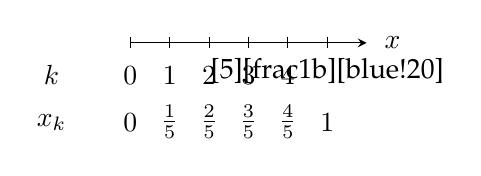
\begin{tikzpicture}[
        ]
        % draw horizontal line   
        \draw[myptr] (0,0) -- (3,0) node[right=3pt] {$x$};
        
        % draw vertical lines
        \foreach \k in {0, 1, 2, 3, 4, 5}
        {
            \ifthenelse{\NOT 0 = \k \AND \NOT 5 = \k}{
                \draw (\k*0.5 cm,2pt) -- (\k*0.5 cm,-2pt)  node[below=3pt] (k\k) {$\k$} node[below=20pt,shift={(0,3pt)}] (xk\k) {$\frac{\k}{5}$};
            }{
                \ifthenelse{5 = \k}{
                    \draw (\k*0.5 cm,2pt) -- (\k*0.5 cm,-2pt)  node[below=3pt,shift={(0,3pt)}] (k\k) {\tfill[5][frac1b][blue!20]} node[below=20pt] (xk\k) {$1$};
                }{
                    \draw (\k*0.5 cm,2pt) -- (\k*0.5 cm,-2pt)  node[below=3pt] (k\k) {$\k$} node[below=20pt] (xk\k) {$\k$};
                }
            }
        }
        \node[left of=k0] {$k$};
        \node[left of=xk0] {$x_k$};
        % draw nodes
    \end{tikzpicture}
    \begin{tikzpicture}[overlay]
        \draw[color=blue!60] (frac1b) -- (frac1);
    \end{tikzpicture}
    
    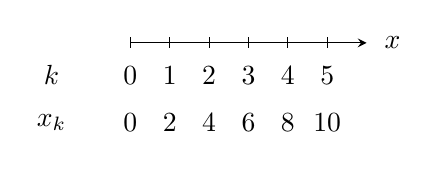
\begin{tikzpicture}[
        ]
        % draw horizontal line   
        \draw[myptr] (0,0) -- (3,0) node[right=3pt] {$x$};
        
        % draw vertical lines
        \foreach \k/\xk in {0/0, 1/2, 2/4, 3/6, 4/8, 5/10}
        {
            \draw (\k*0.5 cm,2pt) -- (\k*0.5 cm,-2pt)  node[below=3pt] (k\k) {$\k$} node[below=20pt] (xk\k) {$\xk$};
        }
        \node[left of=k0] {$k$};
        \node[left of=xk0] {$x_k$};
        % draw nodes
    \end{tikzpicture}

    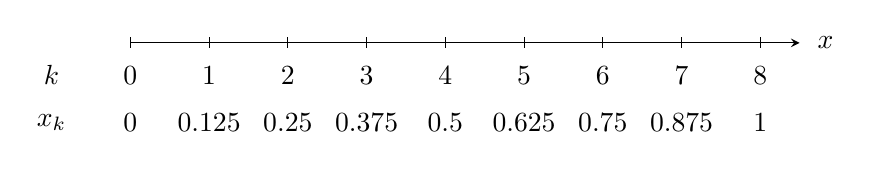
\begin{tikzpicture}[
        ]
        % draw horizontal line   
        \draw[myptr] (0,0) -- (8.5,0) node[right=3pt] {$x$};
        
        % draw vertical lines
        \foreach \k/\xk in {0/0, 1/0.125, 2/0.25, 3/0.375, 4/0.5, 5/0.625, 6/0.75, 7/0.875, 8/1}
        {
            \draw (\k cm,2pt) -- (\k cm,-2pt)  node[below=3pt] (k\k) {$\k$} node[below=20pt] (xk\k) {$\xk$};
        }
        \node[left of=k0] {$k$};
        \node[left of=xk0] {$x_k$};
        % draw nodes
    \end{tikzpicture}



    sss

	\begin{minipage}[t]{0.09\textwidth}
        $x_1$
	\end{minipage}
	\begin{minipage}[t]{0.91\textwidth}
        \begin{align*}
            \gpp[\widetilde{T}][2][2^2][x_1][x_1][x_1] & \\
            \gpp[\widetilde{T}][][2^2][x_2][x_1][x_0] & \\
            \gppn[T_2][T_1][T_0][2^2] & \\
            \gppn[40][T_1][T_0][2^2] &
        \end{align*}
	\end{minipage}

    
    \begin{tabular}{lll}
        \text{{\color{blue}\uline{Hyperpolic}}} & & \text{{\color{red}\uline{Parabolic}}} \\
        $ {\color{blue}r = \f{\dt}{\dx}} $      & ${\color{red}\neq}$ & ${\color{red}r = \f{\dt}{\dx[2]}}$
    \end{tabular}

    

    

    $ \Delta u=u_{xx}+u_{yy}=0 $

    $\Delta u=u_{xx}+u_{yy}=f(x,y)$

    $ \Delta u =  u_{xx} + u_{yy} = \frac{\partial^2 u}{\partial x^2} + \frac{\partial^2 u}{\partial y^2} = 0 $

    \begin{tabular}{ll}
        Nabla Operator                  & $\nabla{u} = u_{x}+u_{y} = \frac{\partial u}{\partial x} + \frac{\partial u}{\partial y}$ \\
        Laplace Operator                & $\Delta{u} = u_{xx} + u_{yy} = \frac{\partial^2 u}{\partial x^2} + \frac{\partial^2 u}{\partial y^2} $\\
        \hline
        \hline
        Anfangswertproblem (AWP)        & \multirow{2}{*}{$u\kl{x,0} = f\kl{x}, \quad {\textstyle\f{\partial u}{\partial x}}\kl{x,0} = g\kl{x}$} \\
        Initial value problem (IVP)     & \\
        \hline
        Randwertproblem (RWP)           & \multirow{2}{*}{$u\kl{x,a} = \alpha, \quad u\kl{x,b} = \beta $} \\
        Boundary value problem (BVP)    & \\
        \hline
        Dirichlet-Randbedingung         & $u\kl{x,0} = f\kl{x}$ \\
        Dirichlet boundary condition    & Werte auf dem Rand liegend \\
        \hline
        Neumann-Randbedingung           & ${\textstyle\f{\partial u}{\partial x}}\kl{x,0} = f\kl{x}$ \\
        Neumann boundary condition      & Ableitungswerte auf dem Rand liegend \\
        \hline
        Laplace-Gleichung               & \multirow{2}{*}{$\Delta u = 0 $}\\
        Laplace's equation              & \\
        \hline
        Poisson-Gleichung               & \multirow{2}{*}{$-\Delta u = f $}\\
        Poisson's equation              &
    \end{tabular}

    \begin{tabular}{lll}
        \multicolumn{3}{c}{$ Au_{xx} + 2Bu_{xy} + Cu_{yy} + Du_x + Eu_y + Fu +G= 0 $} \\
        \hline
        Elliptische PDF                 & Laplace-/Poisson-Gleichung    & \multirow{2}{*}{$ B^2 - AC < 0$} \\
        Elliptic PDE                    & Laplace-/Poisson's equation   & \\
        \hline
        Parabolische PDF                & Wärmeleitungsgleichung, Diffusionsgleichung   & \multirow{2}{*}{$ B^2 - AC = 0$} \\
        Parabolic PDE                   & Heat Equation, Diffusion Equation             & \\
        \hline
        Hyperbolische PDF               & Transportgleichung, Wellengleichung           & \multirow{2}{*}{$ B^2 - AC < 0 $} \\
        Hyperbolic PDE                  & Advection Equation, Wave Equation             &
    \end{tabular}

    \begin{tabular}{ll}
        \hline
        Elliptische PDF                 & Laplace-/Poisson-Gleichung                    \\
        Elliptic PDE                    & Laplace-/Poisson's equation                   \\
        \hline
        Parabolische PDF                & Wärmeleitungsgleichung, Diffusionsgleichung   \\
        Parabolic PDE                   & Heat Equation, Diffusion Equation             \\
        \hline
        Hyperbolische PDF               & Transportgleichung, Wellengleichung           \\
        Hyperbolic PDE                  & Advection Equation, Wave Equation             
    \end{tabular}


    %===================================================================================
    \newpage

    \subsection*{Finite Difference Method (FDM)}
    \subsection*{Elliptic PDEs}

    \subsubsection*{Dirichlet Boundary Conditions}
    
    Discrete Laplace-Operator / 5-Star-Operator
    
    \begin{align*}
        \Delta u & = u_{xx} + u_{yy} \\
        h        & = \dx = \dy \\
        \Delta u & \approx \f{1}{h^2} \kq{u\kl{x + h, y} + u\kl{x, y + h} + u\kl{x - h, y} + u\kl{x, y - h} - 4 \cdot u\kl{x,y}} \\
        \Delta u & \approx \f{1}{h^2} \kq{u\kl{P_E} + u\kl{P_N} + u\kl{P_W} + u\kl{P_S} - 4 \cdot u\kl{P_C}}
    \end{align*}

    \subsubsection*{Neumann Boundary Conditions}

    \begin{align*}
        u_x\kl{P_C} & \approx \f{u\kl{P_E} - u\kl{P_W}}{2\cdot h} \\
        u\kl{P_W}   & = u\kl{P_E} - 2\cdot h \cdot u_x\kl{P_C} \\
        \Delta u    & \approx \f{1}{h^2} \kq{u\kl{P_E} + u\kl{P_N} + \tfillr{$u\kl{P_W}$} + u\kl{P_S} - 4 \cdot u\kl{P_C}} \\
                    & \approx \f{1}{h^2} \kq{u\kl{P_E} + u\kl{P_N} + \tfillr{$u\kl{P_E} - 2\cdot h \cdot u_x\kl{P_C}$} + u\kl{P_S} - 4 \cdot u\kl{P_C}} \\
                    & \approx \f{1}{h^2} \kq{\tfillr{$2$} \cdot u\kl{P_E} + u\kl{P_N} + u\kl{P_S} - 4 \cdot u\kl{P_C} \tfillr{$- 2\cdot h \cdot u_x\kl{P_C}$}} \\
    \end{align*}
    

    
    %===================================================================================
    \newpage

    \subsection*{Parabolic PDEs}
    \subsubsection*{Richardson's Explicit Method}

    \begin{align*}
        u_{t}\kl{x,t}                               & = u_{xx}\kl{x,t} \\
        u_{\dt + 1} & = \ks{\ldots}  u_{\dt}
    \end{align*}
    
    Forward Finite Difference in $t$ and $x$ \\
    {\setlength{\abovedisplayskip}{-6pt}
    \setlength{\belowdisplayskip}{-12pt}
    \begin{align*}
        % 1
        \f{u \kl{x, t + \dt} - \tfillb{$u \kl{x, t}$}}{\dt}    & = \f{
            \tfillr{$u \kl{x + \dx, t}$} -
            2 \cdot \tfillg{$u\kl{x, t}$} +
            \tfilly{$u \kl{x - \dx, t}$}
        }{\dx[2]}, \quad \tfillo{$r$}   = \f{\dt}{\dx[2]}  \\
        % 2
        u \kl{x, t + \dt} & = \tfillo{$r$} \cdot \kq{
            \tfillr{$u \kl{x + \dx, t}$} -
            2 \cdot \tfillg{$u\kl{x, t}$} +
            \tfilly{$u \kl{x - \dx, t}$}
        } + \tfillb{$u \kl{x, t}$} \\
        % 3
        u_{x,t+1} & = \tfillo{$r$} \cdot \kq{u_{x+1,t} - 2 \cdot u_{x,t} + u_{x-1,t}} + \tfillb{$u \kl{x, t}$} \\
        u_{x,t+1} & = \tfillo{$r$} \cdot \tfilly{$u_{x-1,t}$} + \kl{\tfillb{$1$} - \tfillg{$2\cdot r$}} \cdot u_{x,t} + \tfillo{$r$} \cdot \tfillr{$u_{x+1,t}$} \\
        u_{j,k+1} & = \tfillo{$r$} \cdot \tfilly{$u_{j-1,k}$} + \kl{\tfillb{$1$} - \tfillg{$2\cdot r$}} \cdot u_{j,k} + \tfillo{$r$} \cdot \tfillr{$u_{j+1,k}$} \\
        \uline{u}^{k+1} &= C \cdot \uline{u}^{k} \\
        \uline{u}^{k} &= \kq{C}^{k} \cdot \uline{u}^{0}
    \end{align*}}


    \subsubsection*{Richardson's Implicit Method}
    
    Backward Finite Difference in $t$, Forward Finite Difference $x$ \\
    {\setlength{\abovedisplayskip}{-6pt}
    \setlength{\belowdisplayskip}{-12pt}
    \begin{align*}
        % 1
        \f{\tfillb{$u \kl{x, t}$} - u \kl{x, t - \dt} }{\dt} & = \f{
            \tfillr{$u \kl{x + \dx, t}$} -
            2 \cdot \tfillg{$u\kl{x, t}$} +
            \tfilly{$u \kl{x - \dx, t}$}
        }{\dx[2]}, \quad \tfillo{$r$}   = \f{\dt}{\dx[2]}  \\
        % 2
        u \kl{x, t - \dt} & = \tfillb{$u \kl{x, t}$} - \tfillo{$r$} \cdot \kq{
            \tfillr{$u \kl{x + \dx, t}$} -
            2 \cdot \tfillg{$u\kl{x, t}$} +
            \tfilly{$u \kl{x - \dx, t}$}
        } \\
        % 3
        u_{x,t-1} & = \tfillb{$u \kl{x, t}$} -\tfillo{$r$} \cdot \kq{u_{x+1,t} - 2 \cdot u_{x,t} + u_{x-1,t}} \\
        u_{x,t-1} & = -\tfillo{$r$} \cdot \tfilly{$u_{x-1,t}$} + \kl{\tfillb{$1$} + \tfillg{$2\cdot r$}} \cdot u_{x,t} - \tfillo{$r$} \cdot \tfillr{$u_{x+1,t}$} \\
        u_{j,k-1} & = -\tfillo{$r$} \cdot \tfilly{$u_{j+1,k}$} + \kl{\tfillb{$1$} + \tfillg{$2\cdot r$}} \cdot u_{j,k} - \tfillo{$r$} \cdot \tfillr{$u_{j+1,k}$} \\
        \uline{u}^{k} &= E \cdot \uline{u}^{k+1} \\
        \uline{u}^{k+1} &= E^{-1}\cdot \uline{u}^{k} \\
        \uline{u}^{k} &= \kq{E^{-1}}^{k} \cdot \uline{u}^{0}
    \end{align*}}

    \subsubsection*{Method of Crank-Nicolson}
    $\fs{1}{2}$ Explicit, $\fs{1}{2}$ Implicit + $\dt$ \\
    {\setlength{\abovedisplayskip}{-6pt}
    \setlength{\belowdisplayskip}{-12pt}
    \begin{align*}
        % Explicit
        \f{\tfillt{$u \kl{x, t + \dt}$} - \tfillb{$u \kl{x, t}$} }{\dt}    & = \f{
            u \kl{x + \dx, t} -
            2 \cdot u\kl{x, t} +
            u \kl{x - \dx, t}
        }{\dx[2]} \\
        % Implicit + dt
        \f{\tfillt{$u \kl{x, t + \dt}$} - \tfillb{$u \kl{x, t}$} }{\dt} & = \f{
            u \kl{x + \dx, t + \dt} -
            2 \cdot u\kl{x, t + \dt} +
            u \kl{x - \dx, t + \dt}
        }{\dx[2]} \\
        % Method of Crank-Nicolson
        % left
        -\tfillo{$r$} \cdot u_{j-1,\tfilly{$\scriptstyle k+1$}}                 \tfillgr{$+$}
        \kl{2 + 2\cdot \tfillo{$r$} } \cdot u_{j,\tfilly{$\scriptstyle k+1$}}   \tfillgr{$-$}
        \tfillo{$r$}  u_{j+1,\tfilly{$\scriptstyle k+1$}}                       & =
        % right
        \tfillo{$r$} \cdot u_{j-1,\tfillg{$\scriptstyle k$}}                    \tfillgr{$+$}
        \kl{2 - 2\cdot \tfillo{$r$}} \cdot u_{j,\tfillg{$\scriptstyle k$}}      \tfillgr{$+$}
        \tfillo{$r$} \cdot u_{j+1,\tfillg{$\scriptstyle k$}}
    \end{align*}}

    %===================================================================================
    \newpage

    \subsection*{Hyperbolic PDEs}
    \subsubsection*{Advection Equation / Transportgleichung}
    
    {\it{Problem 70}} \\
    \begin{tabular}{p{5cm}l}
        Domain $\dom$                 & $\Omega = \kl{-\infty, \infty} \times \left[ 0, \infty \right)$ \\
        Advection Equation              & $u_x\kl{x,t} + u_t\kl{x,t} = 0$ \\
        Dirichlet boundary-condition on $\bound$    & $u\kl{x,0} = f\kl{x}$
    \end{tabular}

    {\bf{Downwind Scheme}} \\
    Forward Finite Difference in $t$ and $x$ \\
    {\setlength{\abovedisplayskip}{-6pt}
    \setlength{\belowdisplayskip}{-12pt}
    \begin{align*}
        \f{u \kl{x,\;t + \dt} - u \kl{x, t}}{\dt} &+ \f{ \tfilly{$u \kl{x + \dx, t}$} - u\kl{x, t}}{\dx} = 0 \\
        u_{j,k+1} - \tfillb{$u_{j,k}$}  &= \tfillo{${\fs{\dt}{\dx}}$} \kq{u_{j,k} - \tfilly{$u_{j+1,k}$}} \\
        u_{j,k+1}                       &= \tfillo{$r$} \cdot \kq{u_{j,k} - \tfilly{$u_{j+1,k}$}} + \tfillb{$u_{j,k}$} \\
        u_{j,k+1}                       &= \kl{\tfillb{$1$}+\tfillo{$r$}} \cdot u_{j,k} - \tfillo{$r$} \cdot \tfilly{$u_{j+1,k}$}
    \end{align*}}

    {\bf{Upwind Scheme}} \\
    Forward Finite Difference in $t$, Backward Finite Difference in $x$ \\
    {\setlength{\abovedisplayskip}{-6pt}
    \setlength{\belowdisplayskip}{-12pt}
    \begin{align*}
        \f{u \kl{x,\;t + \dt} - u \kl{x, t}}{\dt} &+ \f{u\kl{x, t} - \tfillg{$u \kl{x - \dx, t}$}}{\dx} = 0 \\
        u_{j,k+1} - \tfillb{$u_{j,k}$}  &= \tfillo{${\fs{\dt}{\dx}}$} \kq{\tfillg{$u_{j-1,k}$} - u_{j,k}} \\
        u_{j,k+1}                       &= \tfillo{$r$} \cdot \kq{\tfillg{$u_{j-1,k}$} - u_{j,k}} + \tfillb{$u_{j,k}$} \\
        u_{j,k+1}                       &= \kl{\tfillb{$1$}-\tfillo{$r$}} \cdot u_{j,k} + \tfillo{$r$} \cdot \tfillg{$u_{j-1,k}$}
    \end{align*}}

    {\bf{Centred Scheme}} \\
    Forward Finite Difference in $t$, Centered Finite Difference in $x$ \\
    {\setlength{\abovedisplayskip}{-6pt}
    \setlength{\belowdisplayskip}{-12pt}
    \begin{align*}
        \f{u \kl{x,\;t + \dt} - u \kl{x, t}}{\dt} &+ \f{ \tfilly{$u \kl{x + \dx, t}$} - \tfillg{$u \kl{x - \dx, t}$}}{2 \cdot \dx} = 0 \\
        u_{j,k+1} - \tfillb{$u_{j,k}$}  &= \tfillo{${\fs{\dt}{2 \cdot \dx}}$} \kq{\tfillg{$u_{j-1,k}$} - \tfilly{$u_{j+1,k}$}} \\
        u_{j,k+1}                       &= \tfillo{$\fs{r}{2}$} \cdot \kq{\tfillg{$u_{j-1,k}$} - \tfilly{$u_{j+1,k}$}} + \tfillb{$u_{j,k}$} \\
        u_{j,k+1}                       &= - \tfillo{$\fs{r}{2}$} \cdot \tfilly{$u_{j+1,k}$} + \tfillb{$u_{j,k}$} + \tfillo{$\fs{r}{2}$}  \cdot \tfillg{$u_{j-1,k}$}
    \end{align*}}

    {\bf{Lax-Wendroff Scheme}} \\
    Forward Finite Difference in $t$, Centered Finite Difference in $x$ \\
    {\setlength{\abovedisplayskip}{-6pt}
    \setlength{\belowdisplayskip}{-12pt}
    \begin{align*}
        u_{j,k+1} = A \cdot \tfilly{$u_{j+1,k}$} + B \cdot \tfillb{$u_{j,k}$} + C \cdot \tfillg{$u_{j-1,k}$} \\[0.25cm]
        A = \f{r^2 - r}{2}, \qquad B = 1 - r^2, \qquad C = \f{r^2 + r}{r}
    \end{align*}}
    

    
\end{document}
